\documentclass{article}
\usepackage{graphicx}
\usepackage{fullpage}
\usepackage{amsmath}
\usepackage{color}

\newcommand{\dd}[2]{\frac{\partial\,#1}{\partial\,#2}}
\newcommand{\red}[1]{\textcolor{red}{#1}}

\title{Selecting gain, exposure time, and number of frames for the EXCAM exposure time calculators in analog mode}
\author{Eric, Bijan, Vanessa, Rob, Marie, John K.}

\begin{document}
\maketitle

\section{Introduction}
This is the effective detector model:
\begin{figure}[h]
    \centering
    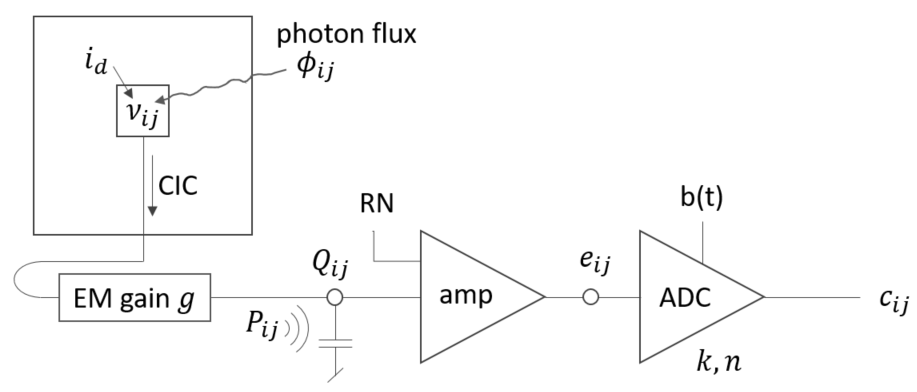
\includegraphics[height=3.8cm]{revisedDetectorModelFigure.png}
    \caption{Detector and readout effective model; see text in following section for explanations of variables.}
    \label{fig:my_label}
\end{figure}
The amplifier has a large gain, but $e_{ij}$ is assumed to be in units of individual electrons, accounting for the amplifier gain. The first amplifier's nonlinearity is assumed to be zero and its bias is constant. Those effects are all lumped into the ADC.
The ADC has conversion gain $k$ and nonlinearity $n$.

At the pixel level, photons are converted to electrons, and there is also dark current ($i_d$). Additionally clocking through to the sense node there is also clock induced charge (CIC), denoted as ($C$).  The electron counts for each pixel in the image area is
\begin{equation}
\nu_{ij} = P_p\left( \phi_{ij}\ \eta_{ij} t_{fr} + i_d t_{fr} + C \right) ,
\end{equation}
where C is the CIC, $P_p$ represents the function that picks a Poisson random variate with mean equal to its argument.

The detector clocks this charge first in parallel direction, then in the serial direction.  Henceforth, we will assume that the total CIC (parallel plus serial) is denoted by $C$ and that the total CIC is just the serial CIC since the parallel CIC is negligible in comparison.  The charge goes through the electron multiplication (EM) gain stage, and the charge is amplified. For a gain $g >> 1$ (set by the clock voltage amplitude) and $n$ electrons going into the gain stage, the output is shown in Basden 2003 to be given by:
\begin{equation}
\label{eq:Basden}
P_\Gamma(x,g)=\frac{x^{n-1}\ e^{-x/g}}{g^n\ (n-1)!}
\end{equation}
This is a special case (integer input and output) of the Gamma distribution function and hence the subscript $\Gamma$.
At the sense node there are EMI pickup effects from the clocking process leading to a "fixed pattern" noise which is pixel dependent, and we label as $p_{ij}$.
\begin{equation}
Q_{ij} = P_\Gamma\left(\nu_{ij}, g \right)  + p_{ij}
\end{equation}
The amplifier adds read noise, which manifests itself as a zero-mean Gaussian variate with standard deviation $\sigma_r$, so we write this as $P_g(\sigma_r)$. Both the output amplifier and the ADC have bias and gain, and the biases can be time dependent and the gains can be nonlinear. In our effective model we assume the amplifier has no bias variation and has a gain of unity, so that its output, in electrons, is:
\begin{equation}
e_{ij} = Q_{ij} + P_g(\sigma_r) \,
\end{equation}

and finally, at the ADC, there is the (effective) bias and the (effective) k gain, and some effective nonlinearity:

\begin{equation}
\label{eq:cts_noav}
c_{ij} = b(t) + \frac{e_{ij}}{k\cdot n} \,
\end{equation}

If we consider an average of many frames, writing it all out, we have:

\begin{equation}
\bar{c}_{ij} = \bar{b} + \frac{1}{k\cdot n}\ \left(p_{ij} + g\cdot (\phi_{ij}\ \eta_{ij} t_{fr} + i_d t_{fr} + C )\right) \,
\end{equation}

We are interested ultimately in $\phi_{ij}$, which we can now relate to the other quantities as:

\begin{equation}
\phi_{ij}\ \eta_{ij} t_{fr} = \frac{k n}{g} (\bar{c}_{ij}- \bar{b}) - \frac{p_{ij}}{g} - i_d t_{fr} - C \,
\end{equation}

We can now define a calibration quantity we will call a  \emph{master dark} $D_{ij}$, as:

\begin{equation}
D_{ij} \equiv  \frac{p_{ij}}{g} + i_d t_{fr} + C \,
\end{equation}

In these terms, the input integrated number of light particles (photons) during an average frame is given by:

\begin{equation}
\label{eq:photons}
L_{ij} \equiv \phi_{ij} t_{fr} = \frac{1}{\eta_{ij}}\left(  \frac{k n}{g} (\bar{c}_{ij} - \bar{b}) - D_{ij} \right) \,
\end{equation}



\section{SNR figure of merit}

\noindent An individual "cleaned" analog-mode EXCAM frame has had the following corrections applied:
\begin{itemize}
\item bias calculation and subtraction: $b(t)$ in DNs, where the $t$ is indicating that the bias changes per frame
\item cosmic ray removal (see below)
\item nonlinearity correction: $n$, unitless
\item dn to e- conversion (k-gain multiplication): $k$, in electrons/DN
\item EM gain division: $g$, unitless
\item dark subtraction (bias-subtracted, gain-corrected): $D_{ij}$ in electrons
\item QE correction: $Q$, electrons/photon (note neglects CTI effects that depend on flux)
\item flat correction: $F_{ij}$, unitless; note $\eta_{ij} = Q F_{ij}$
\end{itemize}
Cosmic-ray removal is not a simple math operation and will be handled separately; the rest can be written in photons/pixel as:
\begin{align}
\label{eq:signal}
    L_{ij} &= \frac{1}{\eta_{ij}}\left(\frac{k n}{g} (\bar{c}_{ij} - \bar{b}) - D_{ij}\right)
\end{align}
Not coincidentally, this is the same as Eq. \ref{eq:photons}; cleaned data nominally returns data in photons.

A mean-combined set of $N$ individual cleaned frames gives the flux at a pixel as:
\begin{align}
\gamma_{ij} = \frac{1}{N} \sum_{m=1}^{N} L_{m}
\end{align}

As a figure of merit for exposure time calculation, we wish to provide an SNR target for the SNR in a pixel of a set of mean-combined cleaned individual frames.  SNR here equals signal/noise, where
\begin{itemize}
\item the signal is the mean number of electrons in a pixel of a set of combined cleaned frames (ensemble mean of $\gamma_{ij}$)
\item the noise is the square root of the variance, in electrons, in a pixel of a set of combined cleaned frames (standard deviation of $\gamma_{ij}$)
\end{itemize}

\subsection{Signal}

Under the assumption that we've done our calibrations right, from Eqs. \ref{eq:photons} and \ref{eq:signal} we can get our signal as
\begin{align}
% \bar{c}_{ij} &= \bar{b} + \frac{1}{k\cdot n}\ \left(p_{ij} + g\cdot (\phi_{ij}\ \eta_{ij} t_{fr} + i_d t_{fr} + C )\right)\\
% \bar{L}_{ij} &= \left(\frac{1}{\eta_{ij}}\left(\frac{k n}{g} (\bar{c}_{ij} -  \bar{b}) - D_{ij}\right)\right) \nonumber \\
% &= \left(\frac{1}{\eta_{ij}}\left(\frac{k n}{g} (\left[\bar{b} + \frac{1}{k\cdot n}\ \left(p_{ij} + g\cdot (\phi_{ij} \eta_{ij} t_{fr} + i_d t_{fr} + C )\right)\right] -  \bar{b}) - D_{ij}\right)\right) \nonumber \\
% &= \left(\frac{1}{\eta_{ij}}\left(\frac{1}{g} \left(p_{ij} + g\cdot (\phi_{ij}\ \eta_{ij}t_{fr} + i_d t_{fr} + C )\right) - \left(\frac{p_{ij}}{g} + i_d t_{fr} + C\right)\right)\right) \nonumber \\
L_{ij} &= \phi_{ij} t_{fr} \\
\gamma_{ij} &= \frac{1}{N} \sum_{m=1}^{N} L_{m} \nonumber\\
&= \frac{1}{N} N \phi_{ij} t_{fr} \nonumber \\
\Rightarrow \gamma_{ij} &= \phi_{ij} t_{fr}
\end{align}
The read noise, $\sigma_{r}$, does not appear in the mean calculations since the read noise is treated as zero-mean--any fixed non-zero mean component will be captured into the fixed pattern, and any per-frame-varying non-zero mean component will be captured in bias estimation.

\subsection{Noise}

To get noise, we go back to Eq. \ref{eq:cts_noav}, and expand it out without averaging:
\begin{align}
c_{ij} = b(t) + \frac{1}{k\cdot n} \left(p_{ij} + P_g(\sigma_r) + P_\Gamma\left(P_p\left( \phi_{ij} \eta_{ij} t_{fr} + i_d t_{fr} + C \right), g \right)\right)
\end{align}
In our detector model above, bias and fixed-pattern do not contribute to variability.  Read noise does, with variance $\sigma_{r}^2$, and all of the combined Poisson processes do as well, with the caveat that the composition of the two distributions $P_\Gamma$ and $P_p$ causes the variance of the overall term to be larger than the variance you would expect from shot noise (Poisson variance) alone.

Without rederiving the analysis here, we will take the approach of Robbins and Hadwen 2003, who define an excess noise factor $F^2$ to model the scaling of the variance as a function of gain $g$ and number of electron-multiplying elements in the gain register $N_{EM}$ (a fixed number = 604 for EXCAM):
\begin{align}
F^2 &= 2(g - 1) g^{-\frac{N_{EM}+1}{N_{EM}}} + \frac{1}{g}
\end{align}
$F^2$ tends approaches 1 as $g \rightarrow 1$, approaches 2 as $g \rightarrow \infty$, and varies smoothly over intermediate gains.  This term will affect only the terms that are enhanced by gain, so read noise does not get excess noise.

We can then get our noise as:
\begin{align}
\sigma_{c_{ij}}^2 &= \frac{1}{k^2 n^2} \left(\sigma_{r}^2 + F(g)^2 g^2 \left(\phi_{ij} \eta_{ij} t_{fr} + i_{d} t_{fr} + C\right)\right) \label{eq:noisec} \\
\sigma_{L_{ij}}^2 &= \sigma_{c_{ij}}^2 \left(\dd{L_{ij}}{c_{ij}}\right)^2 \nonumber \\
\dd{L_{ij}}{c_{ij}} &= \frac{k n}{g \eta_{ij}} \nonumber \\
\sigma_{L_{ij}}^2 &= \left(\frac{k n}{g \eta_{ij}}\right)^2 \frac{1}{k^2 n^2}\left(\sigma_{r}^2 + F(g)^2 g^2 \left[\phi_{ij} \eta_{ij} t_{fr} + i_{d} t_{fr} + C\right]\right) \nonumber\\
\Rightarrow \sigma_{L_{ij}}^2 &= \left(\frac{1}{g \eta_{ij}}\right)^2 \left(\sigma_{r}^2 + F(g)^2 g^2 \left[\phi_{ij} \eta_{ij} t_{fr} + i_{d} t_{fr} + C\right]\right) \\
\sigma_{\gamma_{ij}}^2 &= \sum_{m=1}^N \sigma_{L_{ij, m}}^2 \left(\dd{\gamma_{ij}}{L_{ij, m}} \right)^2 \\
\dd{\gamma_{ij}}{L_{ij, m}} &= \frac{1}{N} \nonumber\\
\Rightarrow \sigma_{\gamma_{ij}}^2 &= \frac{1}{N^2} \sum_{m=1}^N \left(\frac{1}{g \eta_{ij}}\right)^2 \left(\sigma_{r}^2 + F(g)^2 g^2 \left[\phi_{ij} \eta_{ij} t_{fr} + i_{d} t_{fr} + C\right]\right) \nonumber\\
&= \frac{1}{N} \left(\frac{1}{g \eta_{ij}}\right)^2 \left(\sigma_{r}^2 + F(g)^2 g^2 \left[\phi_{ij} \eta_{ij} t_{fr} + i_{d} t_{fr} + C\right]\right)
\end{align}

\subsection{SNR}

Given the signal and noise forms, our SNR can be written as:
\begin{align}
SNR &= \frac{\phi_{ij} t_{fr}}{\sqrt{\frac{1}{N} \left(\frac{1}{g \eta_{ij}}\right)^2 \left(\sigma_{r}^2 + F(g)^2 g^2 \left[\phi_{ij} \eta_{ij} t_{fr} + i_{d} t_{fr} + C\right]\right)}} \nonumber \\
&= \sqrt{N} \frac{\phi_{ij} \eta_{ij} t_{fr}}{\sqrt{\left(\frac{\sigma_{r}^2}{g^2} + F(g)^2  \left[\phi_{ij} \eta_{ij} t_{fr} + i_{d} t_{fr} + C\right]\right)}} \\
 &= \frac{\sqrt{N \phi_{ij} \eta_{ij} t_{fr}}}{F(g)} \frac{1}{\sqrt{1 + \frac{i_{d}}{\phi_{ij} \eta_{ij}} + \frac{1}{\phi_{ij} \eta_{ij} t_{fr}}\left(C + \frac{\sigma_{r}^2}{F(g)^2 g^2}\right) }}
\end{align}

Key takeaways:
\begin{itemize}
\item Cross-check: In the limit where there is no EM gain ($g = 1, F(g) = 1$) and the dark current rate, CIC, and read noise are small compared to the flux, the SNR reduces to $\sqrt{N \phi_{ij} \eta_{ij} t_{fr}}$, which is the expected SNR from a pure photon noise contribution across all frames.
\item Cross-check: In the limit where there is large EM gain ($F(g) \rightarrow \sqrt{2}$), the dark current rate and CIC are small compared to the flux, and read noise is small compared to the flux after compensation by gain, the SNR reduces to $\frac{1}{\sqrt{2}}\sqrt{N \phi_{ij} \eta_{ij} t_{fr}}$, which is the expected SNR from a pure photon noise contribution across all frames divided by the expected EMCCD excess noise factor.
\item The only effects of EM gain are 1) to introduce the excess noise factor, and 2) to compensate for read noise.   Unlike exposure time and number of frames, which increase the SNR in an unbounded way as they go to infinity, the $g \rightarrow \infty$ limit is just the $\sigma_{r} = 0$ case with $F(g) = \sqrt{2}$, and there are very diminishing returns to increasing gain once the read noise term is small compared to other terms in the denominator.
\item The ratio of dark-current electron accumulation to photon-derived electron accumulation provides a second SNR reducing factor $\frac{i_{d}}{\phi_{ij} \eta_{ij}}$, and neither gain nor exposure time nor number of frames can do anything about its effect on the denominator.
\item Exposing longer per frame can help reduce CIC and read noise effects relative to other noise terms; collecting more frames has no effect, positive or negative, on the square root term containing the noise factors.
\item If we assume that cosmic ray compensation is implemented well, and each affected pixel is either fixed perfectly or masked, the effect of the cosmic ray correction is to reduce N.
\item This formulation does not include variance terms due to calibration uncertainty, and so it should be considered an upper bound.  In the absence of calibration uncertainty terms, none of the multiplicative terms (nonlinearity, k-gain, flat fielding) have any effect on SNR; only bias and dark subtraction have an effect by removing common-mode backgrounds.
\end{itemize}

\section{Calculating camera settings for finite numbers of frames in analog-mode observations}

There are additional physical constraints that must be met when selecting a set of camera parameters $(g, t_{fr}, N)$:
\begin{itemize}
\item The only difference between the unocculted and occulted exposure-time calculators is that $\phi_{ij}$ is smaller when viewing a given star occulted rather than unocculted, so we will use the same basic algorithm for both.
\item The mean number of electrons in a detector pixel $(\phi_{ij} \eta_{ij} t_{fr} + i_{d} t_{fr})$ must be less than some maximum value, which will generally be some fraction (up to 1.0) of the full-well capacity (FWC).  May be chosen less than 1.0 for e.g. linearity; we will use $\alpha_0$ for this variable.
\item The mean number of electrons in a detector pixel after gain, $g (\phi_{ij} \eta_{ij} t_{fr} + i_{d} t_{fr} + C)$ must be less than some maximum value, which will generally be some fraction (up to 1.0) of the serial register FWC; this has a separate capacity from a pixel.  May be chosen less than 1.0 for e.g. linearity; we will use $\alpha_1$ for this variable.
\item We want to go a little further here, and allow these bounds to be placed several standard deviations above the mean to permit a user to further bound the possibility of exceedance.  The standard deviation for the image area ($\sigma_{im}$), in electrons, is the square root of the mean number of electrons in a detector pixel, and the standard deviation for the serial register ($\sigma_{ser}$), in electrons, is the gain multiplied by this mean number of electrons, and then multiplied by the extra noise factor:
\begin{align}
\sigma_{im} &= \sqrt{\phi_{ij} \eta_{ij} t_{fr} + i_{d} t_{fr}} \\
\sigma_{ser} &= F(g) g \sqrt{\phi_{ij} \eta_{ij} t_{fr} + i_{d} t_{fr} + C} \\
\end{align}
and the above two full-well constraints in the bullet points become:
\begin{align}
(\phi_{ij} \eta_{ij} t_{fr} + i_{d} t_{fr}) + n_{\sigma} \sigma_{im} &\leq \alpha_{0} FWC \\
g(\phi_{ij} \eta_{ij} t_{fr} + i_{d} t_{fr} + C) + n_{\sigma} \sigma_{ser} &\leq \alpha_{1} FWC_{EM}
\end{align}
for some user-specified $n_{\sigma}$.  Choosing $n_{\sigma} = 0$ reduces these to the previous case in the above bullet points.
\item There is a concern that flux considerations are not uniform.  Specifically, any frame will in general have a brightest pixel, which is driving full-well constraints to avoid saturation/blooming, and this may not be the same as the flux in the pixels of interest for analysis.  (For example, HOWFSC frames sometimes have bright speckles outside the dark hole extent.)  To mitigate this, we define a brightest-pixel flux $\phi_{b} \geq \phi_{ij}$ and use $\phi_{b}$ in the full-well constraints, including $\sigma$, leaving the SNR constraints using $\phi_{ij}$. In some cases, such as observing an unocculted star, we expect those the brightest pixel and the set of pixels of interest to overlap, and $\phi_{b} = \phi_{ij}$.
\item The number of frames that can be taken must be bounded above (49 frames) by the Camera Imaging Electronics (CIE) capacity.  When taking a finite number of frames, the CIE stored them all in an internal buffer before releasing them, and we will not be allowed to ask for more than the CIE can hold. If you need more than 49, you will need multiple calls or need to accept lower SNR.  HOWFSC is straight-up capped at 49 due to the need to clean onboard.
\begin{itemize}
\item Collecting frames continuously actually doesn't have any sort of cap--CIE handles it differently--but it does have a limit on minimum exposure time so that frames aren't falling on top of each other.  This is set by the rate at which the CIE can transfer data to internal SpaceWire.  Calculating settings for continuous mode observations is not covered by this document.
\end{itemize}
\item The number of frames that can be taken should usually be bounded below by some value $> 1$, so that a cosmic ray does not leave an area with no usable data.
\item The exposure time should be bounded below, and this constraint may be set by data rate constraints or Camera Proximity Electronics (CPE) limitations at a value $> 0$.
\item The exposure time should be bounded above by either FWC or by a cap set by e.g. hardware constraints.
\item The gain must be $\geq 1$.
\item The number of data frames should be augmented to take extra frames, to permit the loss of some number of frames to cosmic rays.  The formula for that factor is discussed below
\end{itemize}

\subsection{Cosmic ray corrections}

Cosmic ray arrival rates will follow some probability distribution $P$, with some probability $P(n=0)$ of getting no hits on a given pixel in a given frame.  Given $X$ cosmic ray hits/sec/$m^2$, $a$ $m^2$/pixel, and $t_{fr}$ seconds/frame, we can expect on average $Xat_{fr}$ hits/pixel/frame on EXCAM.

Each hit causes some number of surrounding pixels to be unusable, either due to spill from the cosmic ray hit or from the tail of the cosmic ray.  For any given target pixel there are some $\ell_{ij}$ pixels on the array, including itself, which could make the target pixel unusable if the other pixel was hit and spreads its charge.  For example, we may choose to mask a $1 \times L$ pixel ``tail'' region for each cosmic ray. For a coordinate system where $j$ increases to the right and the tails extend to the left, the tail mask length will be $j$ pixels for $j<L$ and $L$ pixels for $j \geq L$.  $\ell_{ij}$ may thus change depending on where on the detector you are looking, but the map of $\ell$ over all $i,j$ is fixed.  The probability $\Pi$ of getting no hits on any of those $\ell_{ij}$ pixels is $\Pi = P(n=0)^{\ell_{ij}}$.

If we want $N$ good frames, we should expect to take some $M \geq N$ to accommodate some losses.  The probability of getting $N$ good frames when taking $M$ can be taken from the binomial distribution: $R(N; M) = \binom{M}{N} \Pi^N (1 – \Pi)^{M-N}$, and the expected value of this distribution is $M \Pi = M P(n=0)^{\ell_{ij}}$.

To use this further, we need some knowledge of what $P(n=0)$ should be.  We have the expected value of the distribution $E(n) = Xat_{fr}$, but this isn't enough on its own to determine $P(n=0)$.  For the purposes of this calculator, we choose to model the number of cosmic rays in a frame as a Poisson distribution $P(n, \lambda) = \frac{e^{-\lambda} \lambda^{n}}{n!}$; this model is consistent with each cosmic ray arrival being independent of others and of past arrival history.  The mean of the Poisson distribution is $\lambda$, so we can let $\lambda = Xat_{fr}$ and find
\begin{align}
P(n=0) &= e^{-\lambda} =  e^{-Xat_{fr}}\\
M\Pi &= M P(n=0)^{\ell_{ij}} = M  e^{-Xat_{fr} \ell_{ij}} \\
\end{align}
and so to get an expected value of $N$ good frames, you must take at least $N  e^{X a t_{fr} \ell_{ij}}$.

We can feed that back into our SNR calculation to give:
\begin{align}
SNR_{CR}(g, t_{fr}, N) &= \sqrt{N e^{-Xat_{fr} \ell_{ij}}} \frac{\phi_{ij} \eta_{ij} t_{fr}}{\sqrt{\left(\frac{\sigma_{r}^2}{g^2} + F(g)^2  \left[\phi_{ij} \eta_{ij} t_{fr} + i_{d} t_{fr} + C\right]\right)}}
\end{align}
as the expected SNR for a gain/exposure time/number of frames with cosmic ray discounting effects included.

\section{The optimization problem for analog-mode observations}

\noindent Let us define the desired optimization problem as:

\begin{align}
\mathrm{minimize}\, & N t_{fr} \\
\mathrm{subject\,to:} & \nonumber \\
SNR_{CR}(g, t_{fr}, N) & \geq SNR_{target} \\
(\phi_{b} \eta_{ij} t_{fr} + i_{d} t_{fr}) + n_{\sigma} \sqrt{\phi_{b} \eta_{ij} t_{fr} + i_{d} t_{fr}} &\leq \alpha_{0} FWC \\
g(\phi_{b} \eta_{ij} t_{fr} + i_{d} t_{fr} + C) + n_{\sigma} F(g) g \sqrt{\phi_{b} \eta_{ij} t_{fr} + i_{d} t_{fr} + C} &\leq \alpha_{1} FWC_{EM} \\
N_{min} &\leq N \leq N_{max} \\
t_{min} &\leq t_{fr} \leq t_{max} \\
1 &\leq g \leq g_{max}
\end{align}

where we have incorporated the pixel FWC constraint directly into a constraint on $t_{fr}$.  The minimization constraint is chosen to select the set of $(g, t_{fr}, N)$ which minimizes the wall-clock time to collect data, including the need to take extra images to compensate for data loss to cosmic rays.  Solve this optimization problem to get $(g, t_{fr}, N)$ if the optimization is feasible, round up $N$ to the next integer, and return these values.

If the solver finds that the problem is not feasible--there is no $(g, t_{fr}, N)$ which satisfies all the constraints simultaneously--then we define a second, backup optimization that gets the best SNR that we can given the other constraints.  This optimization will

\begin{align}
\mathrm{maximize}\, & SNR_{CR}\left(g, t_{fr}, N\right) \\
\mathrm{subject\,to:} & \nonumber \\
(\phi_{b} \eta_{ij} t_{fr} + i_{d} t_{fr}) + n_{\sigma} \sqrt{\phi_{b} \eta_{ij} t_{fr} + i_{d} t_{fr}} &\leq \alpha_{0} FWC \\
g(\phi_{b} \eta_{ij} t_{fr} + i_{d} t_{fr} + C) + n_{\sigma} F(g) g \sqrt{\phi_{b} \eta_{ij} t_{fr} + i_{d} t_{fr} + C} &\leq \alpha_{1} FWC_{EM} \\
N_{min} &\leq N \leq N_{max} \\
t_{min} &\leq t_{fr} \leq t_{max} \\
1 &\leq g \leq g_{max}
\end{align}


Return the produced $(g, t_fr, N)$ after rounding $N$ up, with a warning that the requested SNR was not achievable, but giving the SNR that could be achieved.

If this second optimization is infeasible as well, then something is wrong with the detector parameters, $\alpha$ values, or source parameters as defined/selected, because there is no possible viable set of camera settings that meets all constraints.  An example would be observing an extremely bright source, such that $\phi_{ij} \eta_{ij} t_{fr} > FWC$ even when $t_{fr} = t_{min}$--in other words, it will always saturate the detector.

There will be an initial viability precheck before running the optimization to catch the obvious pathological cases.  In any event, if the precheck fails or both optimizations are infeasible, raise an exception and exit.

Other use cases for running the optimization include:
\begin{itemize}
\item fixed exposure time (e.g., when flat-fielding)
\item fixed gain (e.g., $g=1$ for safe operation)
\item fixed number of frames (e.g., possibly acquisition or alignment).
\item fixed total exposure time (the product $N t_{fr}$ fixed)
\end{itemize}
The solver is be executed in a similar manner for these use cases.  For these,
the constraints simplify to a subset of constraints.

\end{document}